\ifx\notes\undefined
    \providecommand{\notesroot}{../../..}
    \providecommand{\demoroot}{.}

    \title{强化学习}
    \author{Donald Cheung\\jianzhang9102@gmail.com}
    \date{\today\footnote{文档编写开始于2017年11月11日}}

    \documentclass[a4paper,10pt]{ctexbook}
\usepackage{xeCJK}
\usepackage{fontspec}
\usepackage{minted}
\usepackage[CJKbookmarks,colorlinks,linkcolor=red]{hyperref}
\usepackage{geometry}
\usepackage{amsmath}
\usepackage[format=hang,font=small,textfont=it]{caption}
\usepackage{float}
\usepackage{subfigure}
\usepackage[nottoc]{tocbibind}
\usepackage{bm}
\usepackage[table, x11names, dvipsnames]{xcolor}
\usepackage{color}
\usepackage{array, booktabs, boldline}
\usepackage{cellspace}
\usepackage{longtable}

\setmainfont{Times New Roman}
\setsansfont{Helvetica}
\setmonofont{Courier New}
\setCJKmainfont[BoldFont={SimHei},ItalicFont={SimHei}]{SimSun}
\setCJKsansfont{SimSun}
\setCJKmonofont{SimSun}

\setcounter{secnumdepth}{4}
\setcounter{tocdepth}{4}

\geometry{left=3.0cm,right=3.0cm,top=2.5cm,bottom=2.5cm}
\bibliographystyle{plain}

%%%%%%%%%%%%%%%%%%%%%%%%%%%%%%%%% minted setting %%%%%%%%%%%%%%%%%%%%%%%%%%%%%%%%%%%
\usemintedstyle{monokai}
\definecolor{bg}{HTML}{282828} % from https://github.com/kevinsawicki/monokai
%\defaultfontfeatures{}
\newfontfamily\noligsmonofamily[NFSSFamily=noligsmonofamily]{Courier}
\setminted{fontfamily=noligsmonofamily}

\renewcommand{\theFancyVerbLine}{%
    \sffamily \textcolor{Dandelion}{\scriptsize \oldstylenums{\arabic{FancyVerbLine}}}}

\newenvironment{jcode}[3]
{%
    \VerbatimEnvironment
    \begin{listing}[h]%
    \caption{#2}%
    \label{#3}%
    \begin{minted}[xleftmargin=18pt,
                   mathescape,
                   linenos,
                   numbersep=5pt,
                   bgcolor=bg,
                   frame=lines,
                   framesep=2mm,
                   fontsize=\footnotesize]{#1}%
}
{%
    \end{minted}
    \vspace{-25pt}%
    \end{listing}%
}
\renewcommand{\listingscaption}{代码}%from minted
\renewcommand{\listoflistingscaption}{代码列表}% from minted


\newenvironment{myquote}{\begin{quote}\kaishu\zihao{-5}}{\end{quote}}
\newcommand\degree{^\circ}
\newtheorem{thm}{定理}


\begin{document}
\maketitle
\tableofcontents
\listoflistings

\else
    \providecommand{\demoroot}{\notesroot/tex/template/book}
\fi

\chapter{强化学习}

\section{Q-Learning}

\begin{figure}[ht]
    \centering
    %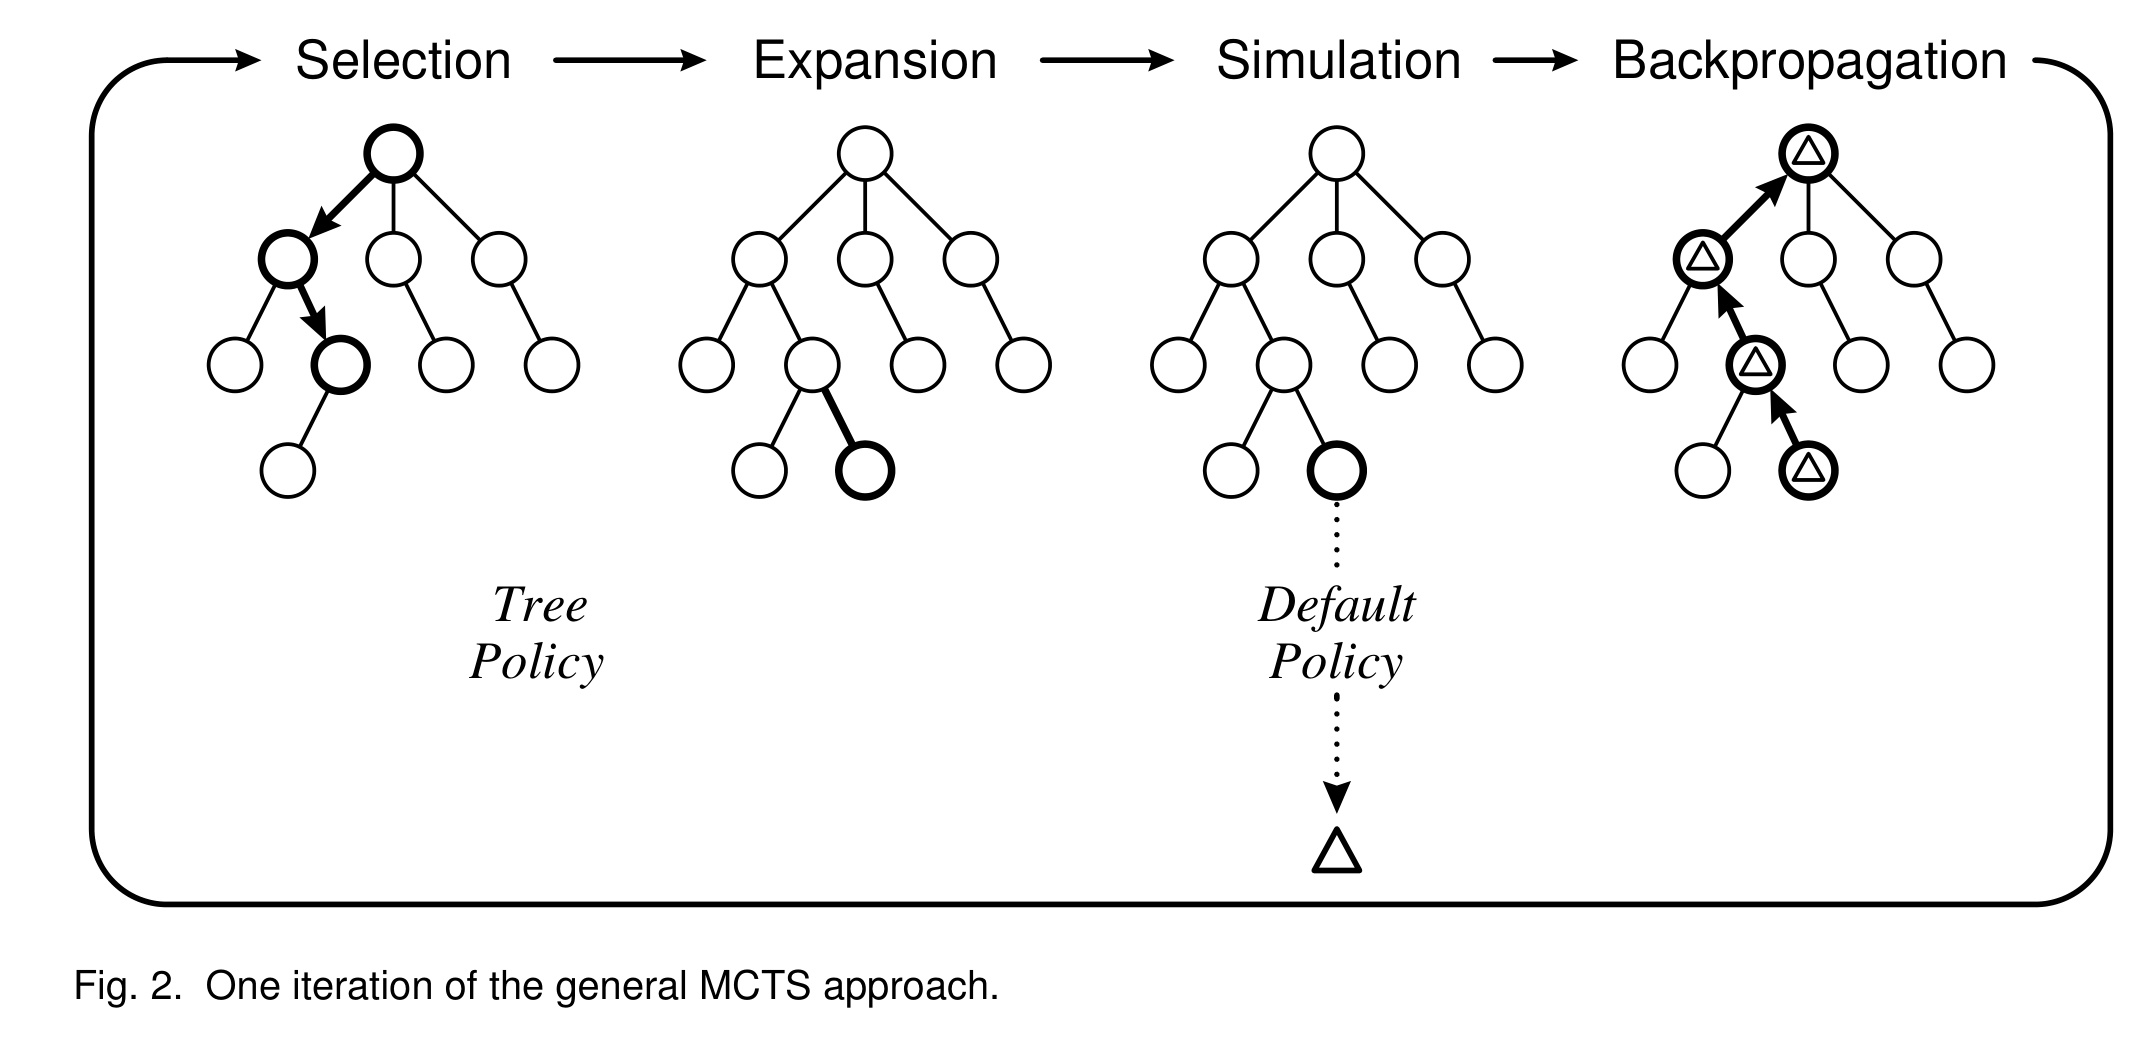
\includegraphics[height=7cm]{\demoroot/images/mcts_approach.jpg}
    \label{fig:mcts_approach}
\end{figure}

\begin{algorithm}
    \SetKwInOut{Input}{Input}
    \SetKwInOut{Output}{Output}

    \underline{function Euclid} $(a,b)$\;
    \Input{Two nonnegative integers $a$ and $b$}
    \Output{$\gcd(a,b)$}
    \eIf{$b=0$}
      {
        return $a$\;
      }
      {
        return Euclid$(b,a\mod b)$\;
      }
    \caption{Euclid's algorithm for finding the greatest common divisor of two nonnegative integers}
\end{algorithm}

\ifx\notes\undefined
    \bibliography{\notesroot/reference/reference.bib}
\end{document}

\fi
